%% tex/deterministic_complexity_classes.tex
%% Copyright 2019 Andrea Berlingieri
%
% This work may be distributed and/or modified under the
% conditions of the LaTeX Project Public License, either version 1.3
% of this license or (at your option) any later version.
% The latest version of this license is in
%   http://www.latex-project.org/lppl.txt
% and version 1.3 or later is part of all distributions of LaTeX
% version 2005/12/01 or later.
%
% This work has the LPPL maintenance status `maintained'.
%
% The Current Maintainer of this work is Andrea Berlingieri.
%
% This work consists of all files listed in manifest.txt
\chapter{Classi deterministiche di complessità}

\section{Macchine di Turing}

La macchina di Turing è un celebre modello di calcolo introdotto in \ref{sec:turingmachine}. Lo
rivediamo qui per comodità in una versione leggermente diversa (multi-tape).

\begin{defn}
    Una Macchina di Turing (multi-tape, deterministica) è una tupla $\tuple{Q, \Gamma, b, \Sigma,
    k, \delta, q_{0}, F}$ dove
    \begin{itemize}
        \item $Q$ è un insieme finito di stati
        \item $\Gamma$ è l'alfabeto finito del nastro
        \item $b$ è il carattere bianco
        \item $\Sigma \subseteq \Gamma \setminus \set{b}$ è l'insieme dei caratteri di input/output
        \item $k \geq 1$ è il numero di nastri
        \item $q_{0} \in Q$ è lo stato iniziale
        \item $F \subseteq Q$ è l'insieme degli stati finali (o di accettazione)
        \item $\delta: Q \setminus F \times \Gamma^{k} \to Q \times \Gamma^{k} \times
        \set{L,R}^{k}$ è la funzione di transizione.
    \end{itemize}
\end{defn}

Intuitivamente abbiamo una serie di nastri con memoria illimitata, divisi in celle di dimensione
fissata. Ogni cella può contenere un carattere di un alfabeto dato, compreso un carattere $b$
(bianco) di inizializzazione. Abbiamo una testina mobile di controllo per ogni nastro ed un automa
di controllo a stati finiti.

Le operazioni fondamentali sono la lettura o scrittura di caratteri individuati dalla testina, lo
spostamento della testina verso destra o verso sinistra, e la modifica dello stato interno
dell'automa.

Per le misure di complessità in genere si tende sempre a prendere come riferimento la macchina di
Turing. Questo perché si tratta di un modello di calcolo semplice in cui sono ben chiari i concetti
di unità di tempo e di unità di spazio, che corrispondono rispettivamente ad una transizione e ad
una cella di memoria.  Ci chiederemo quanti nastri ci permettiamo di usare. Vedremo che questo farà
la differenza.

I nastri sono infiniti, ma in ogni momento si suppone che solo una parte finita del nastro sia stata
scritta. I nastri partono blank, su di essi viene scritto l'input e su di essi si svolge la
computazione.

È la funzione di transizione che governa il comportamento della macchina.

\subsection{Convensioni di input output}

%Slide 47

Si suppone in genere di avere un nastro di input sul quale possono essere effettuate solo letture e
su cui ci si può muovere in una sola direzione. Non è limitante dato che possiamo sempre copiare il
nastro di input in un nastro di lavoro e fare quello che vogliamo sul nastro copia.

Abbiamo anche un nastro di output, di sola scrittura, la cui testina avanza in una sola direzione.

Si suppone in genere di avere già l'input su nastro prima di cominciare la computazione.  Questa
ipotesi non cambia le considerazioni già fatte sulle complessità sublineari, in genere poco
interessanti. Per convenzione supponiamo che la computazione cominci con la testina sul primo
carattere dell'input, con le altre celle che hanno il carattere blank.

Per convenzione supponiamo che, alla fine della computazione, l'output sia la più lunga stringa di
caratteri dell'alfabeto non blank alla sinistra della testina del nastro di output.

È importante non confondere configurazione iniziale e stato iniziale.

\subsection{Configurazioni}

Una configurazione è una descrizione dello stato della computazione ad un dato istante della
computazione.

Rappresentiamo le configurazioni mediante tuple così fatte:
\begin{equation*}
    q, (\sigma_{1},\tau_{1}),\dotsc,(\sigma_{k},\tau_{k})
\end{equation*}
dove $q$ è lo stato dell'automa e $\sigma_{i}$ e $\tau_{i}$ sono due stringhe di caratteri che
descrivono la porzione non (definitivamente) bianca del nastro $i$ alla sinistra e alla destra della
relativa testina. Il carattere in lettura è il primo carattere di $\tau_{i}$.

La computazione avviene per passi discreti: una transizione tra due configurazioni è una relazione
$\vdash$ governata dalla funzione di transizione:
\begin{equation*}
    (q,(\sigma_{1}b_{1},a_{1}\tau_{1}),\dotsc,(\sigma_{k}b_{k},a_{k}\tau_{k})) \vdash
    (q',(\sigma_{1}\beta_{1},\alpha_{1}\tau_{1}),\dotsc,(\sigma_{k}\beta_{k},\alpha_{k}\tau_{k}))
\end{equation*}
se
\begin{itemize}
    \item $\delta(q,a_{1},\dotsc,a_{k}) = (q',a_{1}',\dotsc,a_{k}',D_{1},\dotsc,D_{k})$
    \item se $D_{i} = R$, allora $\beta_{i} = b_{i}a_{i}'$ e $\alpha_{i} = \varepsilon$
    \item se $D_{i} = L$, allora $\beta_{i} = \varepsilon$ e $\alpha_{i} = b_{i}a_{i}'$
\end{itemize}

La relazione $\vdash^{*}$ denota la chiusura transitiva e riflessiva della relazione $\vdash$.

\begin{defn}
    Una funzione $f: \Sigma^{*} \to \Sigma^{*}$ è calcolata da una macchina di Turing $M$ se per
    ogni $\alpha$ esiste $q_{f} \in F$ tale che
    \begin{equation*}
        q_{0}, (\varepsilon,\alpha),\dotsc,(\varepsilon,\varepsilon) \vdash^{*} q_{f},
        (\gamma_{1},\tau_{1}),\dotsc,(\gamma_{k},\tau_{k})
    \end{equation*}
    e $f(\alpha)$ è il più lungo prefisso di $\gamma_{k}$ appartenente a $\Sigma^{*}$
\end{defn}

Detto in altri termini una computazione parte dallo stato iniziale, con i nastri vuoti, con l'input
sul nastro di input e procede per configurazioni succesive, fino ad arrivare ad una configurazione
finale (se la funzione calcolata è definita per il dato input).

\begin{equation*}
    \overequalto{c_{0}}{\varepsilon,q_{0},x} \to c_{1} \to c_{2} \to \cdots \to c_{F}
\end{equation*}

Dato che in complessità noi consideriamo problemi decisionali di solito l'output non è
interessante di per sè. Potremmo avere due stati interessanti, uno di accettazione e uno di
rifiuto.

Nel modello deterministico l'evoluzione della macchina è completamente determinata e univoca per la
macchina considerata dato lo stato iniziale. Lo schema è lineare. La macchina non deterministica
invece non ha una sola mossa disponibile, ne ha un set. Ci possono essere più scelte riguardo alla
mossa successiva.

Lo schema corrispondente smette di essere una sequenza e diventa un grafo, come si puo notare in
figura \ref{img:nondetcomp}.

\begin{figure}[h]
    \begin{center}
        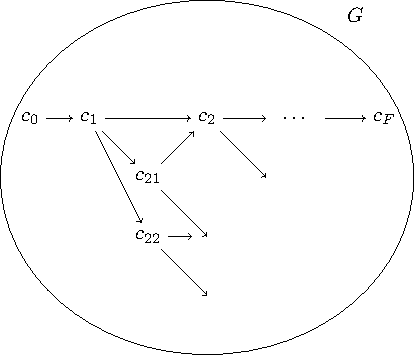
\includegraphics{img/NonDetComputation.pdf}
        \caption{Schema di una computazione non deterministica}
        \label{img:nondetcomp}
    \end{center}
\end{figure}

La computazione della macchina deterministica è un grafo con milioni di nodi. Inoltre questi nodi
sono ``grossi'', un sacco di informazione è codificata in ogni nodo. Questo è un esempio vero di
grafo ``grosso'' (Internet a confronto è un grafo piccolo).

Questo è fondamentale per quanto riguarda la simulazione deterministica della macchina non
deterministica. In sostanza questa si riduce alla visita di tutti i cammini del grafo della
computazione della macchina non deterministica.

Il problema è che dobbiamo visitare tutti i cammini del grafo. Solitamente non basta una visita
semplice. Abbiamo il problema di come svolgere questo processo. Lo rivedremo più avanti.

\section{Classi di complessità}

Prima di vedere le classi di complessità definiamo un pò di operazioni: $\textit{time}_{M}$,
$\textit{space}_{M}$, $t_{M}$, $s_{M}$.

\begin{defn}
    Sia $M$ una Macchina di Turing.
    \begin{itemize}
        \item $\textit{time}_{M}(x)$ è il tempo di esecuzione di $M$ su input $x$: il numero di
        passi richiesti per la computazione
        \item $\textit{space}_{M}(x)$ è il numero massimo di celle visitate da una qualche testina
        durante la computazione (per macchine a più nastri si considerano solo i nastri di lavoro)
        \item $t_{M}(n) := \max\set{\textit{time}_{M}(x) \mid |x| = n}$
        \item $s_{M}(n) := \max\set{\textit{space}_{M}(x) \mid |x| = n}$
    \end{itemize}
\end{defn}

Se in una computazione abbiamo una configurazione $\tuple{\beta, q, \alpha}$ su qualche nastro dove
la lunghezza di $\beta$ e $\alpha$ sono massime, lo spazio consumato è uguale alla somma tra la
lunghezza di $\beta$ e $\alpha$.

Le prime due funzioni calcolano la complessità in funzione dell'input, ma noi vogliamo calcolarla
in funzione della dimensione dell'input. Definiamo quindi le altre due operazioni. $t_{M}$
rappresenta il caso pessimo di complessità in tempo per stringhe di lunghezza $n$. $s_{M}$ è un
analogo per lo spazio.

\begin{defn}
    Sia $f:\Nat \to \Nat$. Definiamo le seguenti classi di complessità:
    \begin{itemize}
        \item $\DTIME(f) := \set{\Lang \subseteq \Sigma^{*} \mid \exists M, \Lang = \Lang_{M} \land
        t_{M} \in O(f)}$
        \item $\DSPACE(f) := \set{\Lang \subseteq \Sigma^{*} \mid \exists M, \Lang = \Lang_{M} \land
        s_{M} \in O(f)}$
    \end{itemize}
\end{defn}

Le classi di complessità sono classi definite in termini di funzioni. La funzione di input mi dà
un ordine di grandezza, non una misura precisa. In altre parole siamo interessati ad $O(f)$.

\textbf{Nota bene:} le classi \textbf{non rappresentano tempi o spazi}. Rappresentano classi di
problemi, o, più formalmente, insiemi di linguaggi.

$\DTIME(f)$ rappresenta l'insieme di linguaggi che sono accettabili da una macchina di Turing in un
tempo $O(f)$.

$f$ è una funzione della dimensione dell'input. $\DTIME(n^{2})$ è l'insieme dei linguaggi che sono
riconosciuti da una MdT in tempo quadratico.

\section{Relazione tra spazio e tempo}

Il teorema che vediamo ora è molto importante. È analogo, a livello di importanza, al problema
della terminazione della teoria della calcolabilità. Ci dice qualcosa sulla relazione tra
complessità in tempo e complessità in spazio.

Sapendo che un certo linguaggio ha una certa complessità in tempo possiamo dire qualcosa sulla sua
complessità in spazio, e viceversa?

Partiamo dalla parte più facile. Supponiamo di avere la complessità in tempo di un algoritmo.

Che motivazioni abbiamo per voler sapere la complessità in tempo? Una è sicuramente che il tempo è
una risora critica. Inoltre è una misura più fine di quella di spazio, ci dà un upper bound a
quest'ultimo. Questo perché se vogliamo aumentare l'occupazione di spazio, con la MdT, dobbiamo
scrivere nuove celle. Sporcare una nuova cella richiede almeno un'unità di tempo. La complessità in
tempo dà un upper bound stretto alla complessità in spazio.

Questo è importante, ed è anche una delle ragioni per cui il tempo è più interessante dello
spazio.

Questo discorso vale a meno di costanti, dato che definiamo noi l'unità di tempo e spazio. Ma una
volta definite queste il ragionamento resta immutato.

Abbiamo quindi che $\DTIME(f) \subseteq \DSPACE(f)$. A prima vista sembrerebbe un'``inversione''. In
realtà se ci pensa se abbiamo un upper bound alla complessità in tempo richiesta per risolvere un
problema abbiamo che lo stesso upper bound si applica per la complessità in spazio, e quindi i
linguaggi di $\DTIME(f)$ fanno sicuramente parte di $\DSPACE(f)$.

\begin{thm}
    Sia $f: \Nat \to \Nat$. Allora $\DTIME(f) \subseteq \DSPACE(f)$.
\end{thm}
\begin{proof}
    Supponiamo che $\Lang \in \DTIME(f)$. Abbiamo quindi che $\exists M, \Lang = \Lang_{M} \land
    t_{M} \in O(f)$. Ma se $t_{M} \in O(f)$ allora anche $s_{M} \in O(f)$. Questo perché il tempo
    è un upper bound allo spazio. Ma quindi $\Lang \in \DSPACE(f)$.
\end{proof}

La D in queste due classi sta per determinstic.

Per dimostrare il teorema abbiamo svolto la nostra analisi sulla stessa macchina. Questo non è
richiesto per la dimostrazione, dato che potremmo immaginare di svolgere la dimostrazione con
un'altra macchina per la parte della complessità in spazio. In questo caso non è stato necessario,
il teorema è puntuale sulla macchina. Se una certa macchina ha una certa complessità in tempo ha la
stessa complessità, al più, in spazio.

Si può occupare anche meno spazio, il tempo fa da upper bound.

Questa era la parte facile, ragioniamo ora sul viceversa. Data la complessità in spazio posso dire
qualcosa sulla complessità in tempo?

Supponiamo ad esempio che una certa macchina di Turing lavori in spazio costante. Quando misuriamo
la complessità in spazio in genere abbiamo macchine multinastro. Di solito non consideriamo lo
spazio del nastro di input. Noi consideriamo solo lo spazio aggiuntivo di cui la macchina ha bisogno
per svolgere la computazione.

In questo ha caso ha senso parlare di complessità sublineari, dato che magari non abbiamo bisogno
di uno spazio aggiuntivo della stessa dimensione dell'input. In particolare possiamo avere spazio
costante, indipendente dall'input.

Un punto importante è che la complessità la misuriamo sempre al termine della computazione. Se la
computazione non termina la complessità è indefinita, quindi non è un caso interessante quello di
loop infinito. Se la complessità è definita non possiamo divergere.

Siamo in loop se passiamo per due volte sulla stessa configurazione. Ma noi questo non lo
permettiamo. Perciò abbiamo un insieme finito di possibili configurazioni che verranno assunte in
una computazione che giunge a termine.

Proviamo a calcolare il numero possibile di configurazioni immaginando di lavorare con uno spazio
costante. Consideriamo i possibili nastri diversi di lunghezza $L$. Questi sono $|\Sigma|^{L}$.
Moltiplichiamo per $|Q|$, il numero di stati. Infine moltiplichiamo per $L$, dato che la testina
potrebbe essere su qualsiasi cella del nasto. Otteniamo la seguente quantità:
\begin{equation*}
    L \times |Q| \times |\Sigma|^{L}
\end{equation*}

Questo rappresenta un upper bound alla complessità in tempo del problema.

Il numero degli stati è fissato in base alla macchina. L'ordine è dato da $L$. La crescita è
esponenziale. Non è così grave, c'è molto di peggio.

Questa analisi vale in caso di complessità costante. Cambia qualcosa se la complessità in spazio
ha un ordine $O(s(n))$? No, basta che la mia $L$ diventi una $L(s(n))$. Il discorso si applica
invariato. Sappiamo che o la macchina termina entro questo upper bound oppure è in loop.

Anche qui l'analisi è puntuale. Data una macchina e una complessità in spazio possiamo dare una
complessità in tempo sulla stessa macchina, non ne dobbiamo produrre un'altra.

In un certo senso per alcuni programmi non possiamo decidere la terminazione perché non possiamo
neanche decidere la quantità di spazio che verrà richiesto. Si può dimostrare che se è decidibile il
problema di sapere qual è l'occupazione di una certa risora sarebbe decidibile il problema di sapere
qualcosa per un altra risorsa. Questo perché tutte le misure di complessità sono correlate. Questa
correlazione può essere pessima a piacere, nel nostro caso era esponenziale.

In questa analisi stiamo dimenticando qualcosa. Sembrerebbe che se abbiamo una complessità in
spazio costante avremmo una complessità in tempo costante, e quindi sublineare. Tuttavia in realtà
noi dobbiamo sapere anche fino a che punto siamo arrivati nell'input. Questo va ad influire sul
numero delle combinazioni. In particolare va aggiunta la lunghezza dell'input alla misura data
prima.
\begin{equation*}
    n\times L \times |Q| \times |\Sigma|^{L}
\end{equation*}

Quindi abbiamo che, se $M \in \DSPACE(f(n))$ allora $\exists c, M \in \DTIME(c^{f(n) + \log(n)})$.
Ricordiamo che $n = c^{\log_{c}(n)}$.

\begin{thm}
    Sia $f: \Nat \to \Nat$. Allora $\DSPACE(f) \subseteq \bigcup_{c \in \Nat}\DTIME(c^{log + f})$.
\end{thm}

Ancora una volta l'esponenziale non è così male. Tutta la teoria della complessità si gioca tra
esponenziale e polinomiale, è un vincolo abbastanza vicino.

\section{Dipendenza dal modello di calcolo}

La macchina di Turing è molto flessibile dato che ci sono tante variabili che possono influire. Ci
chiediamo quanto questo ci influenzi nella nostra analisi.

Se rimpiccioliamo l'alfabeto abbiamo bisogno di stati nuovi per ricordare che ruolo ha un simbolo del
nuovo alfabeto rispetto a quello che aveva nel vecchio.

Lo slowdown è lineare. Se passiamo, ad esempio, da ASCII a binario dovremo fare 8 passi per uno
equivalente. Era di moda tempo fa la ricerca della macchina di Turing universale che minimizzasse la
somma tra grandezza dell'alfabeto e numero di stati.


\subsection{Riduzione dei nastri}

Vediamo qualcosa di più importante, ovvero la riduzione dei nastri.

Immaginiamo di passare da due nastri ad un solo nastro. Perché è problematico lavorare con un
nastro? Immaginiamo di avere una stringa $l$ sul nastro e di volerla copiare più avanti. Con un
nastro solo questa operazione è molto complessa. Dobbiamo leggere i caratteri $x_{0},\dotsc,x_{n}$
uno alla volta, memorizzando il carattere con uno stato interno. Non possiamo memorizzare l'intera
stringa usando uno stato interno perché non abbiamo un upper bound alla lunghezza della stringa.

\begin{figure}[h]
    \begin{center}
        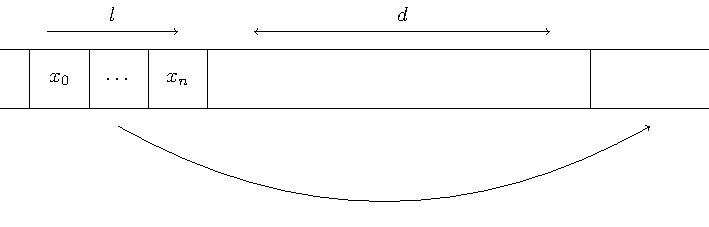
\includegraphics{img/CopyString.pdf}
        \caption{Copia di una stringa con due nastri}
    \end{center}
\end{figure}

Se la distanza è $d$ sono necessari $d\cdot l$ giri avanti e indietro. Essendo $d$ almeno lineare in $l$
(non consideriamo condizioni di overlap) abbiamo complessità almeno quadratica.

Con due nastri è semplice. Basta copiare la stringa di input su un altro nastro, posizionare la
testina del nastro di input dove vogliamo copiare la stringa e posizionare la testina del secondo
nastro all'inizio della stringa. A questo punto è sufficiente scrivere nel primo nastro il
carattere letto dalla testina sul secondo nastro fino a raggiungere la fine della stringa.

\begin{figure}[h]
    \begin{center}
        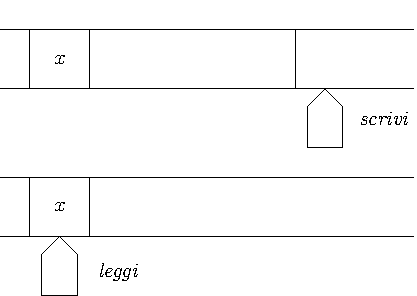
\includegraphics{img/CopyString2Tapes.pdf}
        \caption{Copia di una stringa con due nastri}
    \end{center}
\end{figure}

Passando da due nastri ad uno abbiamo uno slowdown che può essere quadratico. Questo è pesante. La
complessità computazionale dipende dal modello di calcolo. Nell'ambito delle macchine di Turing
questi slowdown restano però polinomiali.

C'è una sottigliezza da considerare riguardo la macchina a due nastri. Le due testine possono
essere lontane a piacere, e il tempo di trasmissione tra le due può quindi aumentare
arbitrariamente. Non è sempre corretto considerare il costo della tramsissione pari ad 1.

%Slide 50

% TODO maybe move this to the part on the size of the input
%Se pensiamo ad $x$ come una stringa $|x|$ corrisponde alla lunghezza della stringa; per i numeri,
%usando una rappresentazione almeno binaria, abbiamo una dimensione $|x|$ uguale a $\log(x)$.

%Slide 51

% TODO move this somewhere more appropriate
% Lo spazio mi da' un upper bound al tempo, ma questo e' molto piu' lasco.

%Slide 52

% TODO move this somewhere more appropriate
%C'e' una dipendenza tra complessita' e modello di calcolo che usiamo.

Generalizzando, proviamo a pensare ad una macchina a $k$ nastri e a come simularla con un nastro
solo. Se avessimo un modo efficiente per fare cio' avremmo un modo generale per eseguire un qualsiasi
algoritmo eseguito sulla macchina a $k$ nastri su un solo nastro. La complessita' dell'emulatore ci
da' un upper bound alla complessita' legato dall'overhead richiesto per la simulazione.

La prima ipotesi che facciamo e' la seguente: non poniamo restrizioni sull'alfabeto dei nastri.
Possiamo pensare di avere un alfabeto molto ricco per la macchina ad un nastro. In particolare
possiamo immaginare di avere a disposizione un alfabeto i cui simboli rappresentano l'unione di vari
pezzi dell'alfabeto originale. E' in un certo senso analogo all'utilizzo di una parola di memoria a
64 bit per memorizzare due parole di memoria a 32 bit. Come abbiamo visto cambiare l'alfabeto
comporta un overhead lineare.

Facciamo poi un'altra ipotesi: da qualche parte dobbiamo memorizzare la posizione della testina.

Noi immaginiamo di simulare $k$ nastri su un nastro solo utilizzando un alfabeto per il nostro
nastro in cui ogni simbolo rappresenta $k$ nastri e $k$ ``tracce''. I simboli sui nastri simulati
sono simboli dell'alfabeto originale, e sulle ``tracce'' memorizziamo la posizione della testina di
ogni nastro rispetto al nastro simulato. In figura \ref{img:KTapesToOne} e' possibile vedere una rappresentazione
grafica di questo processo.

\begin{figure}[h]
    \begin{center}
        % TODO Should probably remake it in Tikz
        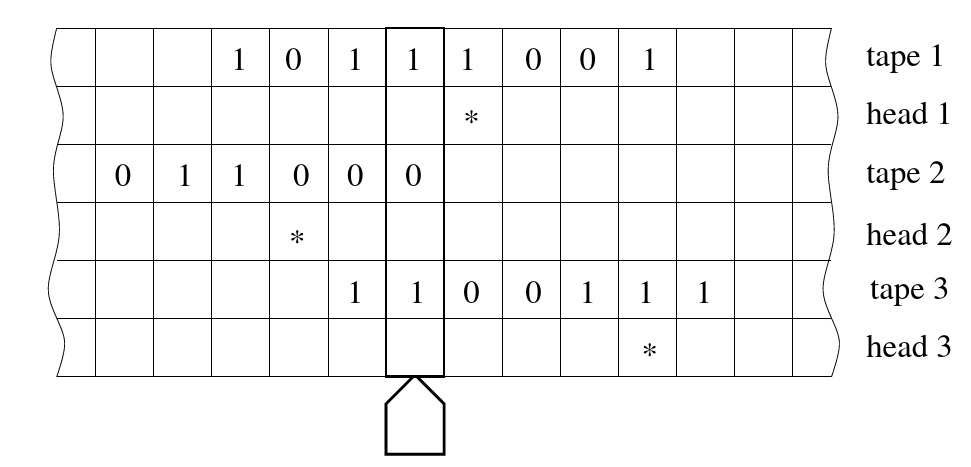
\includegraphics[scale=0.3]{./img/KTapesToOne.png}    
        \caption{Simulazione su una MdT con un nastro di una MdT con piu' nastri}
        \label{img:KTapesToOne}
    \end{center}
\end{figure}

Se $\Sigma$ e' l'alfabeto originale, il nuovo alfabeto e' $\Sigma' = (\Sigma \times
\set{*,B})^{k}$.

Proviamo ora a capire quanto ci costa simulare una operazione della macchina a $k$ nastri su questa
macchina.

Ci sono dei piccoli accorgimenti che si possono fare per avere dei miglioramenti dal punto di vista
della complessita' in tempo, a dispendio della memoria. Ad esempio potremmo immaginare di
memorizzare dell'informazione ulteriore che ci dia una direzione nella quale dovremmo cercare la
testina, in modo da non dover scansionare l'intero nastro. Tuttavia queste ottimizzazioni non sono
significative a livello di complessita'.

Supponiamo di avere due nastri per semplicita'. La nostra macchina sarebbe descritta da $n$-uple
cosi' fatte:
\begin{equation*}
    ((a_{1},a_{2}),q,(a_{1}',a_{2}'),q',(M_{1},M_{2}))
\end{equation*}
dove $a_{1},a_{2}$ sono i caratteri in lettura, $M_{1}$ e $M_{2}$ sono le due mosse sulle testine,
$a_{1}'$ e $a_{2}'$ sono i due nuovi caratteri da scrivere e $q$ e $q'$ rappresentano,
rispettivamente, lo stato attuale e il nuovo stato. Questa e' una tipica istruzione della macchina a
due nastri.

Simulando questa macchina con un nastro solo abbiamo quindi bisogno di una prima passata del nastro
per capire quali sono i caratteri in lettura e salvarli in uno stato interno. A questo punto
riportiamo la testina all'``inizio'' del nastro e facciamo un'altra passata per scrivere i nuovi
caratteri. Infine facciamo una terza passata per simulare la mossa sui nastri simulati.

Sono quindi necessarie piu' passate per simulare un'operazione della macchina a piu' nastri.
Un'operazione che aveva costo 1 ora ha un costo che dipende dall'occupazione di memoria. Possiamo
dare un upper bound alla dimensione del nastro al tempo $t$?  Si', abbiamo un limite lineare in $t$.
Siamo passati da costo 1 a costo $O(t)$. Inoltre il nostro upper bound non e' costante, peggiora col
tempo.

Qual e' il costo totale della simulazione? Abbiamo una somma di operazioni di costo lineare. Di
conseguenza avremo un costo totale quadratico.

Abbiamo quindi visto che con una simulazione fatta in questo modo abbiamo un overhead quadratico.
Non abbiamo pero' dimostrato che passando da $n$ nastri ad un nastro abbiamo necessariamente un
overhead quadratico. Ci potrebbe essere un modo migliore per fare simulazioni che non implica questo
aggravio nella complessita'.

Un altro modo in cui potremmo fare la nostra simulazione e' quello di utilizzare un alfabeto
$\Sigma' = \Sigma^{k}$, se $\Sigma$ era l'alfabeto di partenza, e immaginare di tenere le testine
tutte allineate e che siano i nastri a muoversi sotto le testine.

Con una simulazione fatta in questo modo non dobbiamo piu' cercare la testina, i caratteri in
lettura li troviamo subito, le scritture le facciamo immediatamente. Quello che diventa complicato
e' fare la mossa. Dobbiamo fare una riscrittura dell'intero nastro per fare questo shift dei nastri
simulati. Questo richiede quantomeno una scansione della memoria occupata.

% TODO c'e' un discorso sul fatto che utilizzando 2 testine per la simulazione abbiamo un overhead
% ammortizzato, ma non lo abbiamo visto approfonditamente in classe. Potrebbe essere interessante da
% aggiungere
%
%Passando da $k$ nastri a 2 nastri abbiamo una versione ammortizzata, ma passando ad un nastro solo
%non c'e' modo. (Slide 53)

L'overhead di simulare una macchina a $k$ nastri con una macchina ad un nastro solo sembra quindi
essere intrinsicamente quadratico.

% TODO volendo si potrebbe approfondire il discorso su questo linguaggio non riconoscibile in
% o(n^{2}). La dimostrazione e' interessante

%Slide 59

A riprova di questo fatto esistono linguaggi che sono riconoscibili in tempo lineare con una
macchina a due nastri, in tempo quadratico con una macchina ad un nastro, ma che non sono
riconoscibili in un tempo che sia un $o(n^{2})$ con una macchina ad un nastro. Un linguaggio con
queste caratteristiche e' il seguente:
\begin{equation*}
    \Lang = \set{w\#^{|w|}w \mid w \in \set{0,1}^{*}}
\end{equation*}

La dimostrazione di questo fatto e' interessante perche' e' in generale difficile dimostrare che un
certo problema non si possa risolvere con un algoritmo di complessita' migliore di una nota. La
dimostrazione fa inoltre uso della complessita' di Kolmogorov.

\subsubsection{Nota sugli slowdown}

Nel calcolare gli slowdown prendiamo un'operazione di costo costante e vediamo quanto costa
eseguirla in un altro modo. In questo modo la complessita' dell'altro modo corrisponde allo slowdown
che abbiamo.

Se non abbiamo costo costante dobbiamo fare un'analisi piu' sofisticata. O prendiamo il caso
pessimo, e cosi' diamo un upper bound. Questo pero' potrebbe essere troppo esagerato, e sarebbe il
caso di dare un upper bound definito meglio.

\subsection{Random Access Machine}

Quanto dipende la complessita' dalla modello che utlizziamo? Per rispondere a questa domanda vediamo
un modello di calcolo molto piu' ``liberale'' della MdT: la Random Access Machine (RAM).

In una RAM abbiamo delle celle di memoria tutte indirizzabili, come se fossero dei registri. Di
queste ne abbiamo una quantita' numerabile. Possiamo accedere a queste mediante ``indirizzi'', che
possiamo immaginare per semplicita' esssere dei numeri interi. L'ipotesi forte che facciamo e' che
ogni registro possa avere dimensione illimitata: in ogni registro possiamo scrivere numeri
arbitrariamente grandi.

Abbiamo, tra i vari registri, il program counter, che e' un registro particolare che mantiene la
prossima istruzione da eseguire.

Non e' un modello realistico di complessita', proprio per via di questa ipotesi non realistica.

Usiamo le seguenti notazioni:
\begin{itemize}
    \item $r_{i}$ rappresenta il contenuto del registro $i$-esimo. Utilizziamo il registro $r_{0}$
    come accumulatore;
    \item $i_{j}$ rappresenta il $j$-esimo input;
    \item $k$ rappresenta il program counter.
\end{itemize}
Il comportamento della macchina e' descritto da programmi composti da una sequenza di istruzioni di
uno dei seguenti tipi:
\begin{itemize}
    \item \textsc{read}, che ha due varianti:
    \begin{itemize}
        \item $\textsc{read }j$, con la seguente semantica: $r_{0} \gets i_{j}$ 
        \item $\textsc{read }\uparrow j$, con la seguente semantica: $r_{0} \gets i_{r_{j}}$ 
    \end{itemize}
    \item \textsc{store}, che ha due varianti:
    \begin{itemize}
        \item $\textsc{store }j$, con la seguente semantica: $r_{j} \gets r_{0}$ 
        \item $\textsc{store }\uparrow j$, con la seguente semantica: $r_{r_{j}} \gets r_{0}$ 
    \end{itemize}
    \item $\textsc{load }x$, con semantica $r_{0} \gets x$
    \item $\textsc{add }x$, con semantica $r_{0} \gets r_{0} + x$
    \item $\textsc{sub }x$, con semantica $r_{0} \gets r_{0} - x$
    \item $\textsc{half}$, con semantica $r_{0} \gets r_{0} / 2$
    \item $\textsc{jump }j$, con semantica $k \gets j$
    \item $\textsc{jpos }j$, con semantica \textbf{if} $r_{0} > 0$ \textbf{then} $k \gets j$
    \item $\textsc{jzero }j$, con semantica \textbf{if} $r_{0} = 0$ \textbf{then} $k \gets j$
    \item $\textsc{halt}$, con semantica $k \gets 0$
\end{itemize}

E' molto simile ad un linguaggio Assembler di un tipico calcolatore. Questo e' un modello piu'
vicino alla macchina di Von Neumann rispetto alla MdT. Consideriamo di costo 1 tutte le operazioni
della RAM, indipendentemente dal fatto che lavorino su interi di grandezza arbitraria. Inoltre se
immaginiamo di avere un problema per cui la dimensione dei nostri registri e' sufficiente il modello
risulta abbastanza fedele a quello di Von Neumann, e quindi alla realta'.

Questo e' un modello abbastanza flessibile e generale, e' difficile immaginare di meglio. Questo
giustifica anche l'irrealta' di questo modello.

Quanto ci costa simulare questa macchina con una MdT? 

Abbiamo delle ipotesi. All'inizio della computazione e' caricato in un particolare registro con
l'input, il PC e' settato all'inizio del nostro programma e tutte le altre celle sono memorizzate a
vuoto, non contengono informazione.

Il problema principale e' come gestiamo la memoria di questa macchina nella MdT. Immaginiamo di
usare un nastro della MdT per la simulazione della memoria. Dobbiamo simulare, registro per
registro, il contenuto dei registri. All'inizio abbiamo solo il registro di input con informazione
interessante.

Non sappiamo in che modo saranno scritti i registri della macchina. Ad esempio non possiamo supporre
che avremo accessi sequenziali (prima il primo registro, poi il secondo, ecc.). Un modo semplice per
simulare la memoria e' descrivere ogni registro con due campi: il nome (il numero) e il valore. Ogni
registro corrisponde ad una coppia nome-valore.

\begin{figure}[h]
    \begin{center}
        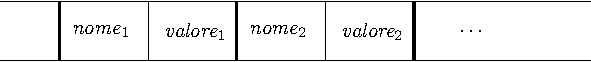
\includegraphics{./img/RAMsimulation.pdf}
        \caption{Simulazione dei regisri di una RAM in una MdT}
    \end{center}
\end{figure}

In generale non possiamo dare un upper bound ne' al numero dei registri ne' alla dimensione di
questi. Potremmo avere un numero arbitrario di registri occupati con valori arbitrariamente grandi.

Sul nastro della memoria memorizziamo le coppie in maniera sequenziale.

Immaginiamo di voler simulare un'operazione, ad esempio la somma. Solitamente si immagina il
registro $r_{0}$ come l'accumulatore utilizzato per le operazioni aritmetiche.

Immaginiamo di sommare, ad esempio, al registro $r_{0}$ il valore del registro $r_{25}$. Dovremo
fare una ricerca in memoria del registro $r_{25}$, leggere il valore e sommarlo al contenuto del
registro $r_{0}$. Non abbiamo problemi di dimensione dell'accumulatore se ad esso dedichiamo un
intero nastro.

Non abbiamo limiti sul numero dei nastri, purche' sia finito. Non possiamo immaginare un nastro per
registro.

Immaginiamo di voler simulare una memorizzazione, magari del risultato della somma. Dobbiamo quindi
scrivere un nuovo valore al posto del valore del registro $r_{0}$. Dovremmo quindi fare delle
operazioni ulteroiri per simulare la memorizzazione, ad esempio uno shift delle coppie nome-valore
verso destra per fare spazio.

Quello che facciamo e' una cosa brutale: cancelliamo il registro (nome-valore) e lo riscriviamo in
fondo. Ha lo stesso costo dello shift, ovvero quello di una scansione della memoria.

\begin{figure}[h]
    \begin{center}
        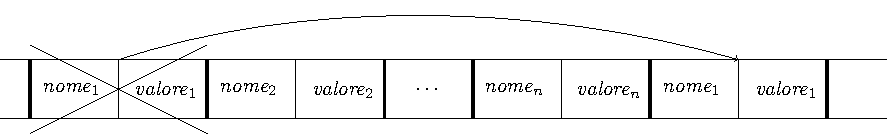
\includegraphics[scale=0.75]{./img/RAMstore.pdf}
        \caption{Simulazione di una memorizzazione in una MdT}
    \end{center}
\end{figure}

Con questo approccio abbiamo problemi di frammentazione e un'occupazione di memoria maggiore
rispetto a quella che avremmo con lo shift, ma in termini di complessita' questo non fa alcuna
differenza.

Cosa possiamo dire sulla dimensione della memoria al tempo $t$ della macchina simulata? Ci chiediamo
quanti registri possiamo avere e quanto questi possono essere grandi.

Il numero di registri referenziati e' limitato da $O(t)$. Quant'e' l'occupazione massima di questi
registri? Sempre $O(t)$. Perche'? Abbiamo una sola operazione che aumenta i valori dei registri, e
quindi l'occupazione di memoria: la somma. Abbiamo che la somma di due numeri di dimensione $n$ puo'
avere al piu' dimensione $n+1$. Di conseguenza, al tempo $t$, abbiamo una occupazione al piu'
quadratica della memoria della macchina simulata.

Simulare una operazione della RAM ci costa quindi $O(t^{2})$. Il costo complessivo della somma sara'
la somma dei $t^{2}$ per $t$ che va da 1 a $t_{\textit{fin}}$. Abbiamo quindi un costo totale
$O(t^{3})$.

Simulare una RAM con una MdT puo' portare ad uno slowdown cubico. Potrebbe andare meglio, ma nel
caso pessimo abbiamo questa complessita'. Questa inoltre potrebbe peggiorare se facessimo la
simulazione con un solo nastro.

Possiamo vedere questo risultato in maniera positiva o negativa. Da un certo punto di vista questo
slowdown e' gravoso. Dall'altro questo slowdown e' comunque polinomiale. In ogni caso un algoritmo
che su RAM aveva complessita' polinomiale se simulato con una MdT continuera' ad avere una
complessita' polinomiale.

Questo e' vero per un modello di calcolo molto liberale. Di conseguenza la complessita'
computazionale di un algoritmo dipende dal modello di calcolo, ma se un modello e' ``ragionevole''
la complessita' dell'algoritmo rimarra' polinomiale anche su questo. La classe polinomiale dei
problemi e' quindi una classe relativamente stabile rispetto al modello di calcolo con cui la
studiamo.

Questo e' vero entro i limiti di ragionevolezza. Cosa intendiamo? Supponiamo di avere come primitiva
anche l'operazione di moltiplicazione. Quello che succede e' che nella simulazione l'occupazione di
memoria esplode: diventa esponenziale. Questo perche' con la moltiplicazione l'occupazione di
memoria puo' crescere di $n$ con un'operazione, dato che il prodotto di numeri di dimensione $n$ ha
puo' avere dimensione $2n$. Avremmo un overhead esponenziale.

E' quindi importante che il modello che utilizziamo abbia un minimo di ragionevolezza. Non ha senso
contare 1 il costo dell'operazione di moltiplicazione. In un certo senso e' gia' strano che
l'addizione abbia costo 1, ma nella RAM lo ammettiamo, e questo si rivela non causare problemi.

Abbiamo quindi due conclusioni importanti:
\begin{itemize}
    \item la complessita' computazionale dipende dal modello di calcolo;
    \item se usiamo modelli di calcolo ragionevoli la complessita' computazionale su di essi non
    differisce piu' che polinomialmente.
\end{itemize}

C'e' chi parla di generalizzazione della tesi di Church, dove alla calcolabilita' corrisponde la
complessita' polinomiale e ai modelli Turing completi corrispondono modelli di calcolo ragionevoli.
Tuttavia questo dipende troppo dalle assunzioni che facciamo sul modello di calcolo, e quindi non ha
la generalita' e lo spessore della tesi di Church.
